\chapter{App messaggistica in Wi-fi Direct}

\begin{minipage}{12cm}\textit{In questo studio di tesi è stata sviluppata un'app per
    dispositivi android che prevede lo scambio di messaggi criptati tra due dispositivi, 
    nei paragrafi seguenti andremo a illustrarne il funzionamento e analizzeremo
    i principali limiti del Wi-Fi Direct in android.}
\end{minipage}




\section{Wi-Fi Direct in android}



Google ha annunciato il supporto Wi-Fi Direct su Android 4.0 a ottobre 2011 
\cite{wikiDi} e si trova su tutte le versione di android successive.
Le specifiche del Wi-fi Direct, come abbiamo visto nel capitolo 3,
non vietano ad un dispositivo di partecipare a più gruppi contemporaneamente.
Tuttavia allo stato attuale in Android  un dispositivo non 
può far parte di due o più gruppi
nello stesso istante di tempo,
di consequenza la fase di discovery deve essere riavviata 
prima della della connessione.

Il Wi-Fi P2P su Android a livello implementativo, è composto da un insieme di
funzioni disponibili al programmatore, chiamate API e che sono divise in tre parti
principali:

\begin{figure}
    \centering
    \caption{metodi principali della classe WifiP2pManager}
    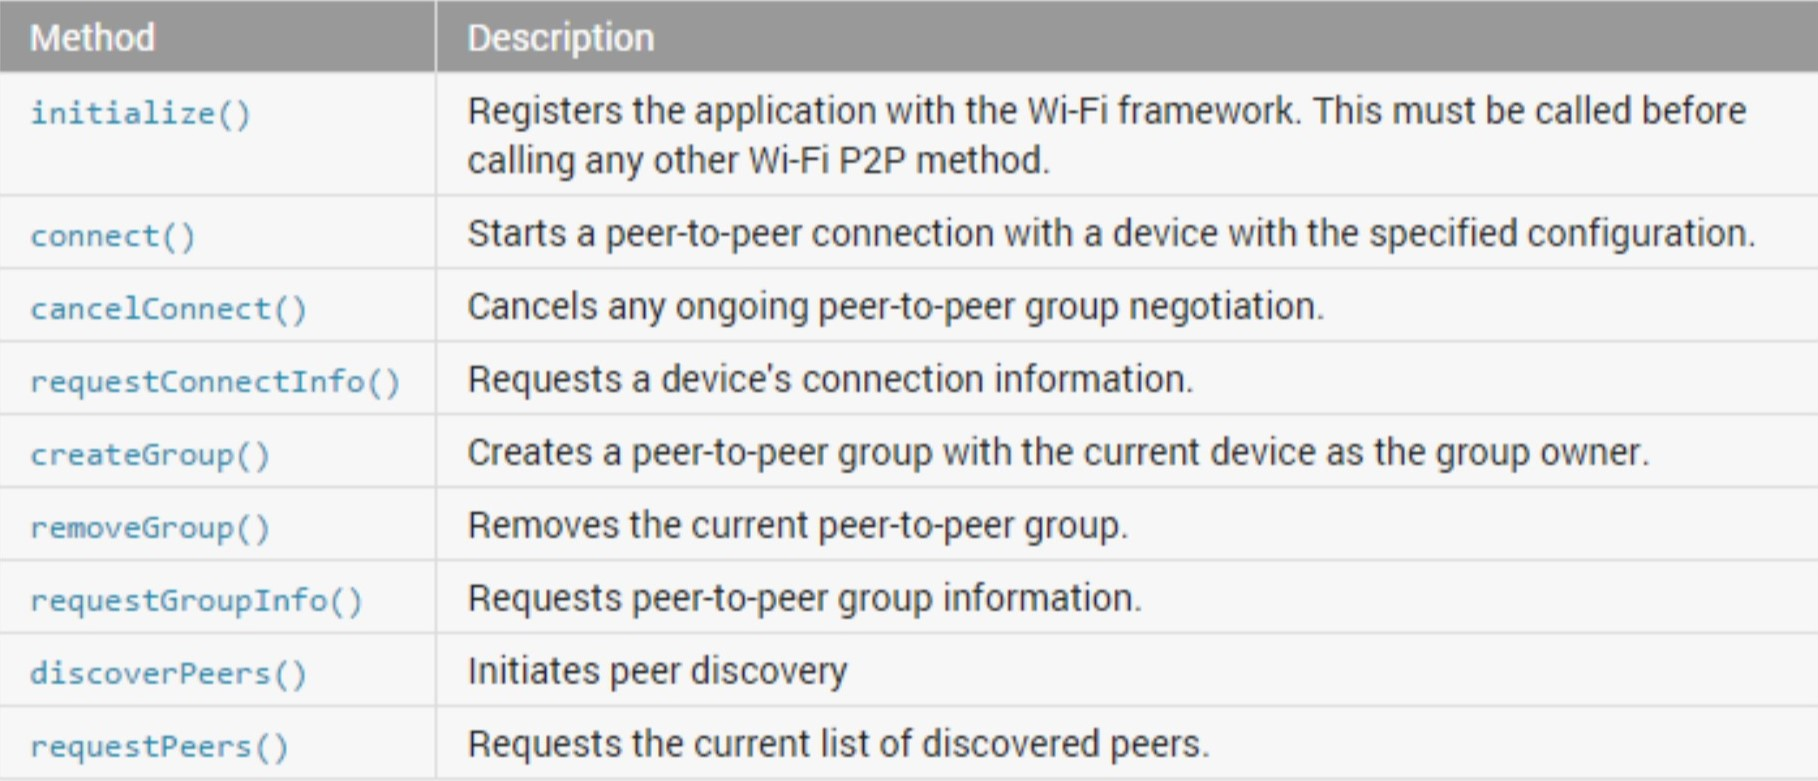
\includegraphics[width=1\columnwidth]{imgs/wifip2pmanagerMet.jpg} 
\end{figure}

\begin{itemize}
    \item tutti i metodi definiti nella classe WifiP2pManager che consentono la scansione,
    richiesta e connessione con i peer;
    \item i listener, “oggetti” che permettono di notificare stati di “successo” o
    “fallimento” quando si eseguono metodi della classe WifiP2pManager;
    \item Intent che notificano per ogni specifico evento rilevato dal device, come ad
    esempio se la connessione cade, se un peer è stato appena scoperto ecc.
\end{itemize}
Qui di seguito in figura, sono esposti i metodi della classe WifiP2pManager.
Ogni metodo della classe WifiP2pManager è collegato a un listener, il quale a
seconda dell’esito della chiamata del metodo, si occupa di avvisare con un
messaggio di successo o fallimento.
Inoltre le APi di Wi-Fi P2P definiscono degli intent che, registrati su un
BroadcastReceiver, permettono all’applicazione di rilevare gli eventi che
accadono in un preciso istante.
\begin{figure}
    \centering
    \caption{lista dei listener associati ai vari metodi della classe WifiP2pManager}
    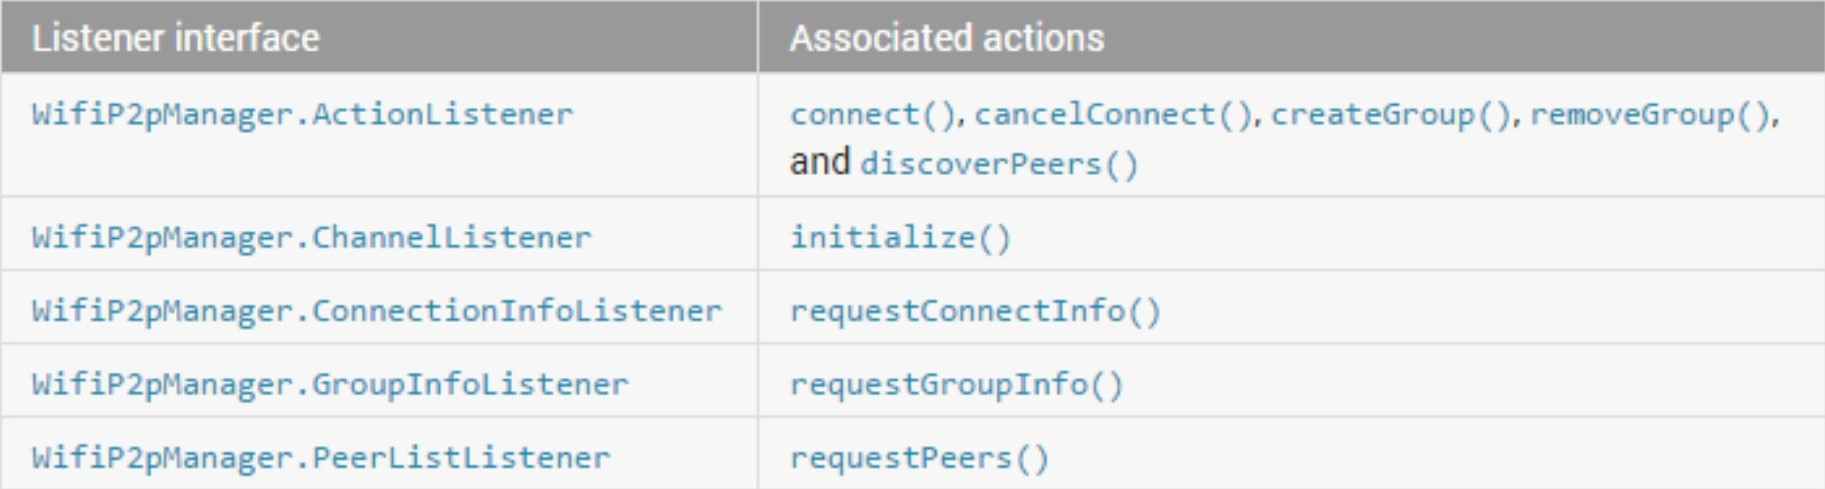
\includegraphics[width=1\columnwidth]{imgs/listenerwifip2pmanager.jpg}
\end{figure}




\section{Funzionamento}
\begin{figure}
    \centering
    \caption{inizio fase di scan}
    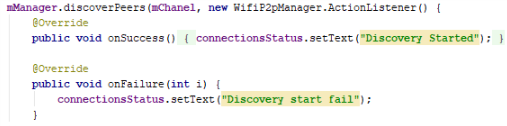
\includegraphics[width=1\columnwidth]{imgs/discoveryStart.png} % Example image
\end{figure}
ho utilizzato le API di Android Software Development Kit (SDK)
\cite{ASD} in Android Studio \cite{ASD} per lo sviluppo di questa applicazione
\subsection{Descrizione alto livello}


L'applicazione prevede la comunicazione tra due dispositivi android,
quest'ultimi eseguono uno scan e una volta che si sono trovati 
possono instaurare una connessione,
che una volta stabilita aprirà un canale di comunicazione bidirezionale tra i due.
I due dispositivi adesso possono scambiare i messaggi.
\subsection{Fase di scan}
\begin{figure}
    \caption{listener dei peer}
    \centering
    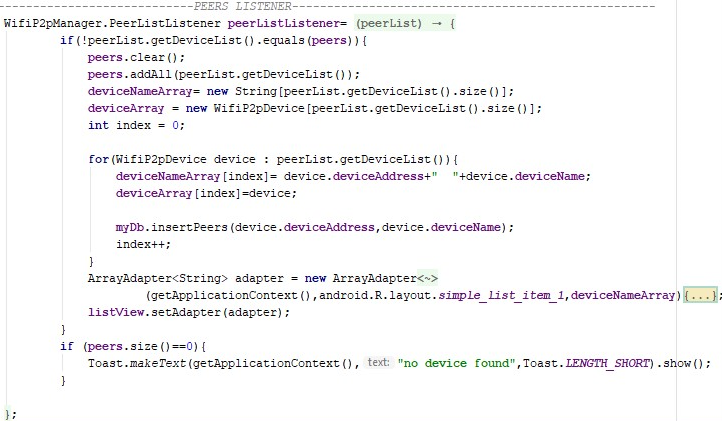
\includegraphics[width=.49\columnwidth]{imgs/peerListener.png}% Example image
\end{figure}

per iniziare la fase di scan si utilizza mManager, un
oggetto che abbiamo istanziato nella MainActivity
di tipo WifiP2pManager,questa classe ci fornisce le API per gestire le connessioni
Wi-Fi P2P \cite{androiddevelopers},
come possiamo vedere dalla figura 3.1.
Per ricavare la lista dei peer (dispositivi vicini)
 si utilizza un listener, 
che ogni volta rileva un nuovo peer lo salva nel suo database 
interno al dispositivo e lo 
visualizza su schermo insieme agli altri, il codice è mostrato
 in figura 3.2


\subsection{Instaurazione della connessione e selezione del Go}



Una volta che l'utente ha su schermo la lista dei dispositivi
vicini può scegliere il dispoitivo con il quale comunicare
semplicemente cliccandoci sopra il dispositivo proverà a 
connettersi al device selezionato usando il metodo "connect" 
della classe "WifiP2pManager" si vede dalla figura 3.3.
\begin{figure}
    \caption{richiesta connessione}
    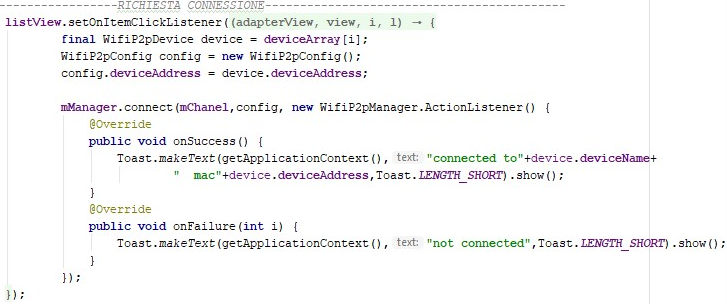
\includegraphics[width=1.4\columnwidth]{imgs/Connect.png}
\end{figure}

Dopo di che entra in gioco il listener della connessione.
in quest'ultimo verà scelta la classe da avviare 
(client o server)in base al dispositivo che è 
diventato GO come si vede nel codice in figura 3.4.

\begin{figure}
    \caption{}
    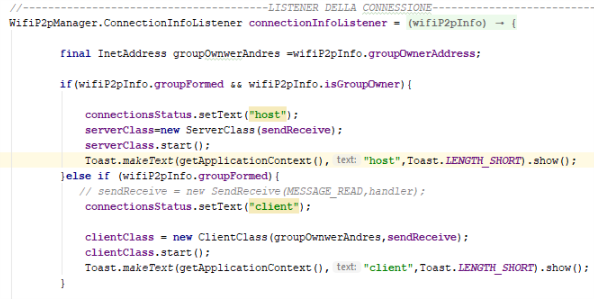
\includegraphics[width=1.2\columnwidth]{imgs/listenerConeessione.png}
\end{figure}

\subsection{Scambio di messaggi}
\subsubsection{Server Class}
Nel caso al dispositivo assume il ruolo del GO
viene istaziato un oggetto della  classe ServerClass,
che accetta una connessione sulla porta 8888 
attraverso una serverSocket che sara utilizzata per comunicare 
attraverso la classe SendReceive come vedremo più avanti 

\begin{figure}
    \caption{server class}
    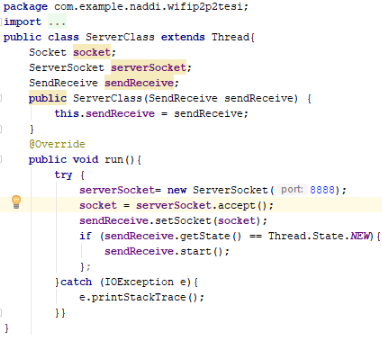
\includegraphics[width=0.6\columnwidth]{imgs/serverClass.png}
    \centering
\end{figure}


\subsubsection{Client Class}
Invece nel caso il dispositivo non assume il ruolo del GO
viene istanziato un oggetto della classe ClientClass,
che prova a connettersi all'indirizzo del GO sulla porta 8888 attraverso
una socket che sara utilizzata per comunicare
attraverso la classe SendReceive come vedremo più avanti.
    
\begin{figure}
    \caption{client class}
    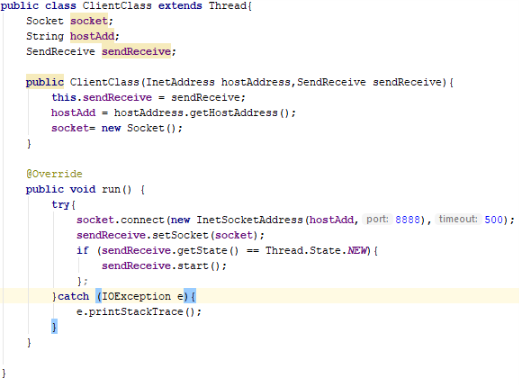
\includegraphics[width=0.7\columnwidth]{imgs/clientClass.png}
    \centering
\end{figure}


\subsubsection{Scambio di messaggi attraverso SendReceive}
SendReceive si occupa di inviare i messaggi all'altro dispoitivo 
e di ricerverli;
per inviarli utilizza il metodo write che scrive 
sull'output stream della socket
per riceverli controlla continuamente con un ciclo l'input stream
della socket


\subsection{Crittografia usata}
Sebbene Wi-Fi Direct utilizza Wpa2 che usa una crittografia di tipo AES 
nell'app si è voluto aggiungere un ulteriore layer di crittografia implemetato a livello
software.
Per criptare i messaggi è stata usata la libreria 
Spongy Castle \cite{Spongy} questa libreria è stata derivata
da Bouncy Castle inquanto  
la piattaforma Android sfortunatamente viene 
distribuita con una versione ridotta di Bouncy Castle, 
Spongy Castle è uguale a Bouncy Castle 
ma con un paio di piccole modifiche per farlo funzionare su Android.
per generare la coppia di chiavi ho usato la curva ellitica con parametri 
(Standards for Efficient Cryptography)
"secp224k1" \cite{sec}.
Per gestire la crittografia è stata creata una classe Cript che contiene
gli oggetti e i metodi necessari per essa: la coppia di chiavi publica e privata 
del dispositivo e la chiave publica dell'altro dispositivo; per quanto rigurda i metodi
invece ce ne sono 4: 
\begin{itemize}
    \item Cript() è il costruttore della classe Cript e
    inizializza la coppia di chiavi publica e privata. 
    \begin{figure}
        \caption{costruttore della classe Cript}
        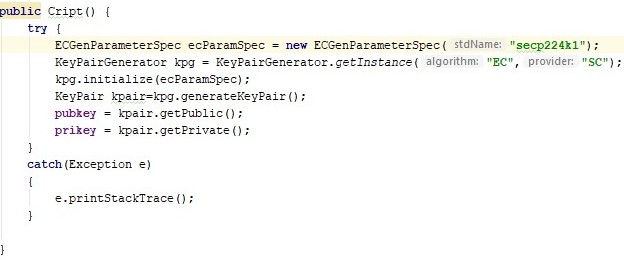
\includegraphics[width=0.8\columnwidth]{imgs/Criptconstructor.jpg}
    \end{figure}

    \item setHisKey() prende in input la chiave publica dell'altro dispsitivo
    encodata in base64 ne fa il decode la memorizza all'interno dell'oggetto
    nel campo "hispub".
    \begin{figure}
        \caption{setter del campo hispub}
        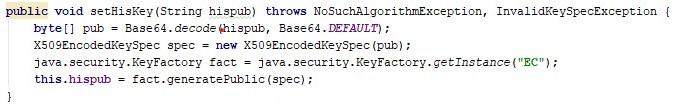
\includegraphics[width=0.9  \columnwidth]{imgs/sethiskey.jpg}
    \end{figure}



    \item encript() prende in input il messaggio da criptare e lo cripta con la
    chiave publica dell'altro dispositivo e ritorna il messaggio criptato
    encodato in base64.
    \begin{figure}
        \caption{metodo per criptare il messaggio}
        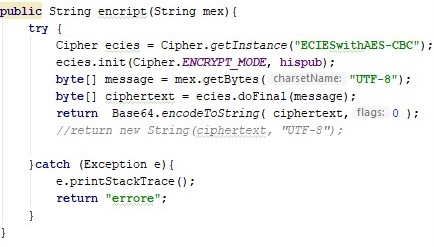
\includegraphics[width=0.5  \columnwidth]{imgs/encript.jpg}
    \end{figure}

    \item decript() prende in input il messaggio da decriptare encodato in base64 
    e lo decripta con
    la sua chiave privata e ritorna il messaggio decriptato.
    \begin{figure}
        \caption{metodo per decriptare il messaggio}
        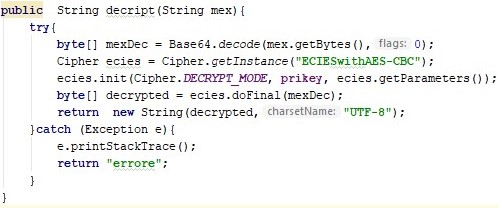
\includegraphics[width=0.6  \columnwidth]{imgs/decript.jpg}
    \end{figure}



\end{itemize} 

\subsubsection{scambio chiavi publiche dei dispositivi} 
Una volta che I dispositivi si sono connessi e hanno istanziato
rispettivamente la classe server e client sono pronti a scambiarsi i messaggi
e il primo messaggio che si scambiano in modo automatico è la loro chiave publica
questo senza che l'utente si accorga di nulla.
la coppia di chiavi publica e privata vegono generate a ogni nuova connessione.


\section{Analisi del Wi-Fi Direct}

Dall'esperienza aquisita sviluppando questo protitipo di app è emerso 
che il Wi-Fi Direct risulta ottimo per connettere i dispositivi singolarmente
fornendo velocità di trasmissione standard del wifi questa cosa è stata confermata
dai test effettuati sul campo che mostremo più avanti, 
mentre non è adatto a formare una rete di dispositivi connessi inquanto
come già spiegato in precedenza in android non è permessa la connessione
del dispoitivo a due Gruppi differenti nello stesso momento.
Dai test si è osservato che il tempo di discovery e quello di formazione del gruppo
hanno mostrato risultati discordanti inquanto con l'aumento della distanza quest'ultimi
impiegavano meno tempo, si noti però che durante lo svilppo dell'app di messaggistica
in alcuni casi la fase di discovery è arrivata a richiedere anche più 10 secondi.
I test che ho fatto inoltre hanno mostrato il limite della portata
del Wi-Fi Direct si è osservato che fino a 64 metri
(all'aperto e senza ostacoli) i dispositivi
si connettevano e riuscivano a scambiare messaggi  mentre a 128 metri
mentri sebbene i disponibili si connettavano non riuscivano
a mantenere la connessione non riuscendo di fatto a scambiarsi messaggi.
Di seguito riporteremo i vari test sulle varie distanze con i tempi (in secondi)di:
discover,group formation,e trasferimento di un paylod da 10MByte.
Un altro limite del Wi-Fi Direct è il consumo di una batteria che risulta
essere elevato.

\subsubsection{I test effettuati}
I test sono stati effettuati attraverso un'app sviluppata da me
su due dispositivi rispettivamente,
uno xiaomi redmi 5 pro e uno xiaomi redmi note 6, pro dove tengo
traccia rispettivamente del tempo che i due dispositivi impiegano a 
trovarsi, il tempo di formazione del gruppo e il tempo che impiegano
per inviare una paylod di 10 MByte.
I test sono stati eseguiti per le seguenti distanze in metri 0,4,8,16,64,128
per ogni distanza il test è stato eseguito 5 volte 
i valori che riporteremo sono la risultatnte della media dei 5.
il test viene eseguito nel seguente: modo chiameremo d1 il dispoitivo 1
e d2 il dispositivo 2,
d2 entra per primo in modalità discovery dopo di che anche d1 entra in modalità
discovery adesso il tempo che d1 impiega per trovare d2 sarà il tempo 
di discovery che viene registrato. Per tempo di formazione del 
gruppo si intende il tempo che uno dei due dispositivi impiga a
diventare Group owner, una volta che i dispositivi sono connessi
si procede con l'invio del payload e registrazione del tempo impiegato.

%https://www.tablesgenerator.com/latex_tables
\begin{table}[]
    \centering
    \begin{tabular}{|c|c|c|c|}
    \hline
    \begin{tabular}[c]{@{}c@{}}Distanze\\ in\\  metri\end{tabular} & \begin{tabular}[c]{@{}c@{}}Tempo\\ (in secondi)\\ Discovery\end{tabular} & \begin{tabular}[c]{@{}c@{}}Tempo\\ (in secondi)\\ formazione \\ gruppo\end{tabular} & \begin{tabular}[c]{@{}c@{}}Tempo\\ (in secondi)\\ invio \\ payload\\ di 10 Mbyte\end{tabular} \\ \hline
    0                                                              & 2.42                                                                     & 1.84                                                                                & 2.5                                                                                           \\ \hline
    4                                                              & 1.45                                                                     & 1.27                                                                                & 5.25                                                                                          \\ \hline
    8                                                              & 1.04                                                                     & 0.94                                                                                & 5.8                                                                                           \\ \hline
    16                                                             & 0.1                                                                      & 1.44                                                                                & 12.4                                                                                          \\ \hline
    32                                                             & \multicolumn{1}{l|}{}                                                    &                                                                                     &                                                                                               \\ \hline
    64                                                             & \multicolumn{1}{l|}{}                                                    &                                                                                     &                                                                                               \\ \hline
    128                                                            & \multicolumn{1}{l|}{}                                                    &                                                                                     &                                                                                               \\ \hline
    \end{tabular}
    \end{table}

\section{Conclusioni}
In questa tesi inizialmente si è visto cosa è una Near-Me area network e
si è fatta un apanoramica sulle reti peer to peer come si correlassero
con il Wi-fi Direct; successivamente siamo andati ad approfondire le specifiche
dello standard del Wi-Fi Direct andando ad analizzarne il
 funzionamento vero e proprio.
Dopo questa parte si è passati allo studio del Wi-Fi Direct
in android e la spiegazione dell'implementazione
proposta di un'app ,svliuppata per questo studio di tesi,
che usa il Wi-Fi Direct per lo scambio di messaggi 
tra due dispotivi.
Successivamente siamo andati a testare le performance del Wi-Fi Direct
atraverso un'altra app sviluppata appositamente per lo scopo.
Da questo studio di tesi è emerso che allo stato attuale 
non è possibile costruire una rete peer to peer
attraverso il Wi-Fi Direct ma più tosto è più orientato
per connessioni peer to peer.
\section{Sviluppi futuri}





